\normalfalse \difficiletrue \tdifficilefalse
\correctionfalse

%\UPSTIidClasse{11} % 11 sup, 12 spé
%\newcommand{\UPSTIidClasse}{11}

\exer{Banc d'épreuve hydraulique $\star$ \label{B2:07:53}}
\setcounter{question}{0}\UPSTIcompetence[2]{B2-07}
\index{Compétence B2-07}
\index{Schéma-blocs}
\index{Banc d'épreuve hydraulique}
\ifcorrection
\else
\marginnote{\textbf{Pas de corrigé pour cet exercice.}}
\fi

\ifprof
\else

\subsubsection*{Analyse de la fonction technique << mettre le tube sous pression >>.}

Un schéma hydraulique simplifié est donné figure suivante.
\begin{center}
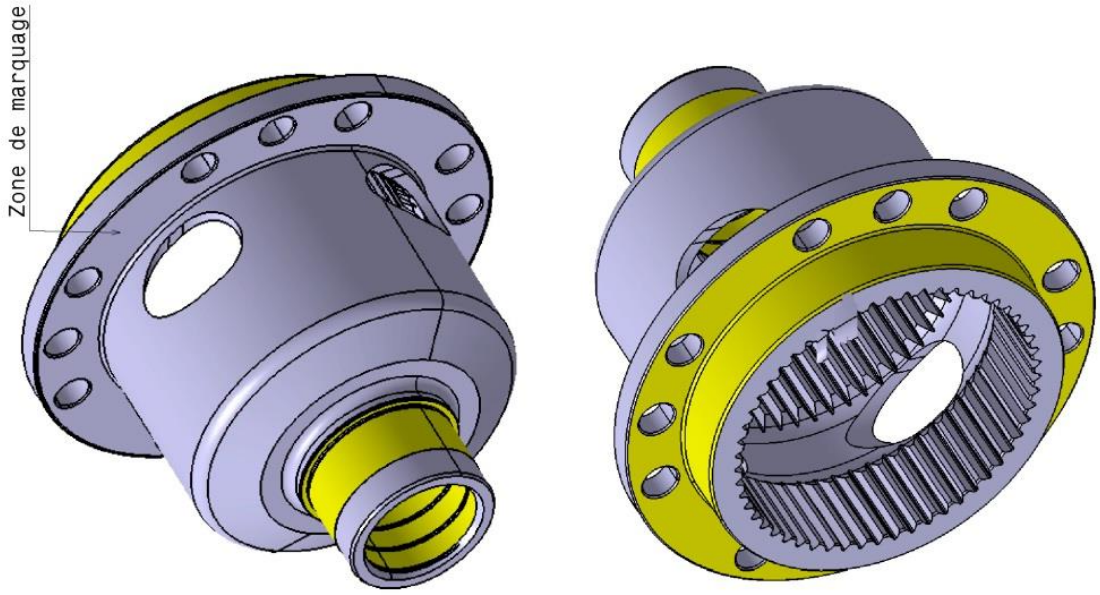
\includegraphics[width=\linewidth]{fig_01}

\end{center}


\subsubsection*{Mise en place du modèle}

Les équations du débit sont : 
$$Q_e(t)=S_e\dfrac{\dd z(t)}{\dd t} - \dfrac{V_{e0}}{B_e}\dfrac{\dd P_e(t)}{\dd t}$$ et 
$$Q_h(t)=S_h\dfrac{\dd z(t)}{\dd t} + \dfrac{V_{h0}}{B_h}\dfrac{\dd P_h(t)}{\dd t}.$$

En appliquant le théorème de la résultante dynamique selon $\vect{z}$ sur le piston du multiplicateur, on a : 
$
M\ddot{z}(t)=S_hp_h(t)-S_ep_e(t)-Mg-f\dot{z}(t).
$

\fi
\question{Déduire de la relation précédente l’équation reliant $Z(p)$, $P_e(p)$, $P_h(p)$, et $\text{Poids}(p)=Mg/p$, transformées de Laplace de $z(t)$, $P_e(t)$, $P_h(t)$ et du poids perçu comme une perturbation. Les conditions initiales sont supposées nulles.}
\ifprof

$Mp^2 Z(p))=S_hP_h(p)-S_eP_e(pt)-\dfrac{Mg}{p}-fpZ(p)$

\else
\fi


\ifprof
\else
On note :
\begin{itemize}
	\item $L(t)$ la position de l’équipage mobile repérée par rapport à sa position initiale;
	\item $V_t(t)$ le volume du tube;
	\item $F_t(t)$ l’effort du tube sur l’équipage mobile, avec $F_t(t) = - rL(t)$.
\end{itemize}

On néglige les variations de volume du tube dues à ses déformations. L’équation du débit s’écrit alors :
	$$Q_e (t)=(S_a-S_b ).\dfrac{\text{d}L(t)}{\text{d}t}+\dfrac{V_t}{B_e}  \dfrac{\text{d}P_e (t)}{\text{d}t}.$$

L’équation du mouvement de l’équipage mobile est donnée par : 
$$
m\ddot{L}(t)=-rL(t)+\left(S_a-S_b \right)p_e(t)-f'\dot{L}(t).
$$
\fi

\question{En déduire, en tenant compte de l’équation du débit, deux équations liant $L(p)$, $P_e(p)$ et $Q_e(p)$, transformées de Laplace de $L(t)$, $P_e(t)$ et $Q_e(t)$. Les conditions initiales sont supposées nulles.}
\ifprof

$Q_e (p)=(S_a-S_b )p L(p)+\dfrac{V_t}{B_e}  p P_e(p)$ et 
$mp^2{L}(p)=-rL(p)+\left(S_a-S_b \right)P_e(p)-f'p{L}(p)$.

\else

\fi

\question{Compléter le schéma-blocs de l’ensemble (sans le distributeur hydraulique), l’entrée étant la pression d’huile régulée $P_r(p)$ et la sortie la pression d’épreuve dans le tube $P_e(p)$.}
\ifprof

\else
\fi

\ifprof
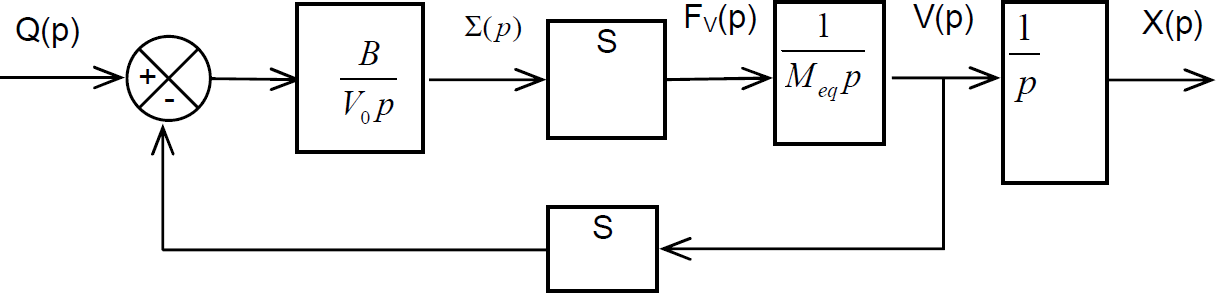
\includegraphics[width=\linewidth]{cor_01}
\else
\begin{center}
\rotatebox{90}{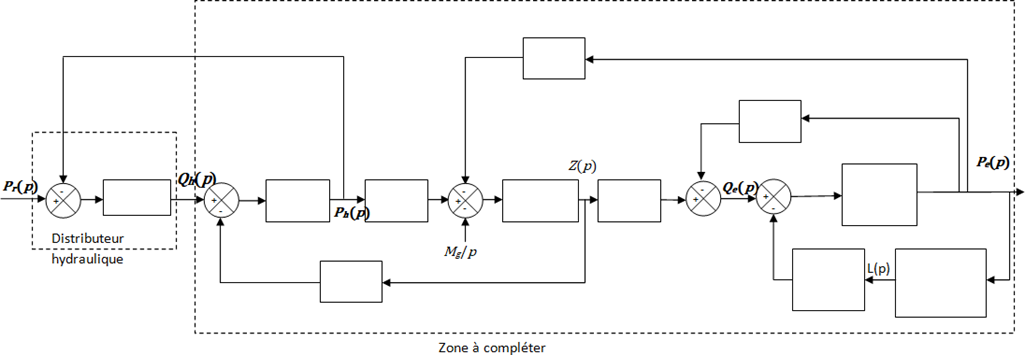
\includegraphics[height=.8\linewidth]{fig_10}}
\end{center}
\fi
 

\ifprof
\else
\begin{flushright}
\footnotesize{Corrigé  voir \ref{B2:07:52}.}
\end{flushright}%
\fi